\documentclass{mylib/reporteConCalif}
\usepackage{float}

\title{Reporte}
\author{rodrigofranciscopablo }

\subject{Laboratorio de Diseño Digital}
\mytitle{Reporte de práctica 5}
\mysubTitle{Minimización de funciones por mapas de Karnahugh}
\students{Francisco Pablo \textsc{Rodrigo}}
\teacher{M.I. Guevara Rodríguez \textsc{Ma. del Socorro}}
\group{6}
\deliverDate{18 de marzo de 2019}

\newcommand{\insertImage}[3]{
	\begin{figure}[H]
		\centering
		\includegraphics[width=#3cm]{#1}
		\caption{#2}
	\end{figure}
}

\begin{document}

\coverPage

\tableofcontents
\newpage

\section{Objetivos}

\subsection{General}

El alumno diseñará circuitos combinacionales.

\subsection{Particular}

El alumno analizará, diseñará e implementará multifunciones, con funciones no especificadas,
optimizando las funciones por medio de mapas de karnahugh.

\section{Introducción}

Un mapa de Karnaugh (también conocido como tabla de Karnaugh o diagrama de Veitch, abreviado como Mapa-K o Mapa-KV) es un diagrama utilizado para la simplificación de funciones algebraicas Booleanas. El mapa de Karnaugh fue inventado en 1953 por Maurice Karnaugh, un físico y matemático de los laboratorios Bell.

El mapa de Karnaugh consiste en una representación bidimensional de la tabla de verdad de la función a simplificar. Puesto que la tabla de verdad de una función de N variables posee 2N filas, el mapa K correspondiente debe poseer también 2N cuadrados. Las variables de la expresión son ordenadas en función de su peso y siguiendo el código Gray, de manera que sólo una de las variables varía entre celdas adyacentes. 

El mapa de Karnaugh se va completando colocando los unos “1” en la celda apropiada, ayudados por la tabla de verdad. Esta agrupación
es conocida como minitérminos o minterms y como expresión booleana viene a ser una suma de productos. Usualmente no se escriben los ceros
“0” en la tabla, ya que solo se agrupan los unos “1”.

\begin{figure}[H]
	\centering
	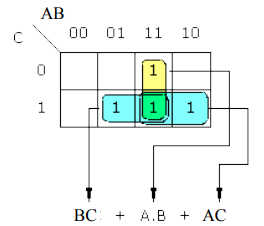
\includegraphics[width=8cm]{img/labdise_pract5/mapa-kv}
	\caption{Mapa de Karnaugh para una función de tres variables.}
\end{figure}

\newpage
\section{Previo}

\newpage
\section{Desarrollo}

Para el desarrollo de ésta práctica tuvimos que utilizar 4 variables de entrada (A,B,C,D) lo cual nos permite tener 16 combinaciones distintas que posteriormente nos servirián para controlar nuestro display de 7 segmentos que puede mostrar números del cero al nueve. Es decir, tenemos 16-10 números sin usar por lo cual los tendremos que considerar don't care.\\

Después de obtener las 7 funciones mínimas las ingresamos al programa \textit{Xilin} para poder hacer la simulación. Para meter las funciones utilizamos el modo HDL y nos quedo lo siguiente.\\

\insertImage{img/labdise_pract5/image1}{Funciones en código VHDL}{15}

Luego, para estar seguros de que ibamos por el rumbo correcto procedimos a hacer la simulación y a corroborar cada una de las combinaciones. 

\insertImage{img/labdise_pract5/image2}{Simulación de nuestro circuito.}{15}

\insertImage{img/labdise_pract5/image4}{Simulación de nuestro circuito.}{15}

Una vez que verificamos que todas las combinaciones de las variables de 4 bits son correctas procedemos a cargar nuestro programa a la FPGA. En este caso para ello abrimos el programa llamado \textbf{Digilent Adept} y en la opción de FPGA escogemos el archivo .bit que generamos en Xilinx y le damos click en \textit{PROGRAMAR}.

\insertImage{img/labdise_pract5/image3}{Cargando el programa a al FPGA}{10}

Finalmente podemos corroborar de manera tangible que nuestro circuito funciona y que la tabla de verdad corresponde con las funciones que programamos.

A continuación se presentan algunas fotos ilustrando el funcionamiento del circuito. Mi número de cuenta es 314331122 por lo cual solo muestro que el 3, 1, 4 y 2 funcionan.

\insertImage{img/labdise_pract5/dos}{El número 2 en el display de 7 segmentos}{12}

\insertImage{img/labdise_pract5/tres}{El número 2 en el display de 7 segmentos}{12}

\insertImage{img/labdise_pract5/cuatro}{El número 2 en el display de 7 segmentos}{12}


\section{Conclusiones}

Obervamos que la mínimización de funciones booleanas es necesaria en el diseño de circuitos lógicos ya que nos ahorra gran cantidad de compuertas si hablamos de elementos físicos o nos ahorra mucho código si hablamos en términos del VHDL y de una FPGA.\\

Es importante mencionar que si no tuvieramos la FPGA tendriamos que implementar nuestro circuito usando solo compuertas lógicas (AND, OR, etc.) y un display de 7 segmentos. Además se complicaría ligerante porque tenemos que tener cuidado al momento de conectar las compuertas con el display ya que este puede ser de ánodo o de cátodo. En cambio, al hacer nuestro programa en XIlinx y el la \textit{Basys} sencillamente programamos nuestro circuito y si veíamos que los números se desplegaban al revés (es decir, se apagaban los que debían estar prendidos) lo único que debimos hacer fue negar nuestras funciones y volver a cargar el programa.

\end{document}